\section{Introduction}
This paper is about an academic project born to be an efficient solution for the CINI\footnote{Consorzio Interuniversitario Nazionale per l'Informatica} 2017 Challenge on smart cities illumination systems. In particular, the goal was to prototype and test a solution which was capable of (near) real-time data stream processing for monitoring records from streetlamps, lumen sensors co-located with the streetlamp itself and from traffic data produced by third-party APIs. We will explore this solution for the following use case: in a smart city context it is necessary to guarantee the maximum efficiency from lamps consumption while providing an optimal illumination within safety limits for pedestrians and drivers and according to local traffic intensity. To achieve that, it is necessary to project a grid of smart lamps capable of tuning their light level according to the right amount of energy necessary to provide city aware, safe and green consumption levels. This grid must be powered and managed via a reliable, highly available, processing-capable control system. Introducing Project Ember.

\section{Frameworks and Tools}

\section{Architecture overview}
In this section we will cover how the system communicates between each of its components and modules and the assumptions we made to prototype and test the architecture. In \hyperref[fig:ember_architecture]{figure 1} a high-level architecture overview is provided. Before proceeding, we want to focus on the output from the real-time\footnote{We will define the system as "real-time" in this paper even if is not validated for such a control system, but it is capable of near real-time data streams processing} control system: it is produced into the MOM\footnote{Messages Oriented Middleware} and consumed by control units (how will be discussed later), closing a feedback loop. This behavior and the capabilities to maintain high-availability across the clusters make the system itself near to the features of an autonomic system.
\begin{figure}
\begin{center}
	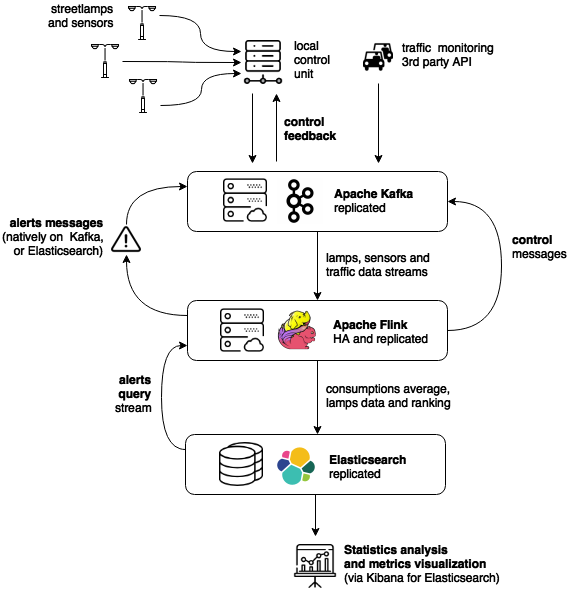
\includegraphics[scale=0.35]{img/ember_architecture}
	\caption{Project Ember architecture overview}
	\label{fig:ember_architecture}
\end{center}
	
\end{figure}


\subsection{Sensors network}
First of all let we consider how the sensors network [...]

% to insert a simple bar chart
%\begin{tikzpicture}
%\begin{axis}[
%	x tick label style={
%		/pgf/number format/1000 sep=},
%	ylabel=Year,
%	enlargelimits=0.05,
%	legend style={at={(0.5,-0.1)},
%	anchor=north,legend columns=-1},
%	ybar interval=0.7,
%]
%\addplot 
%	coordinates {(2012,408184) (2011,408348)
%		 (2010,414870) (2009,412156) (2008,415 838)};
%\addplot 
%	coordinates {(2012,388950) (2011,393007) 
%		(2010,398449) (2009,395972) (2008,398866)};
%\legend{Men,Women}
%\end{axis}
%\end{tikzpicture}